\documentclass[conference]{IEEEtran}

\usepackage{cite}
\usepackage{amsmath,amssymb,amsfonts}
\usepackage{graphicx}
\usepackage{textcomp}
\usepackage{booktabs}
\usepackage{array}
\usepackage{multirow}
\usepackage{tikz}
\usetikzlibrary{arrows.meta,positioning,shapes.geometric,fit,calc}
\usepackage{url}
\usepackage{microtype}
\usepackage[T1]{fontenc}

\def\BibTeX{{\rm B\kern-.05em{\sc i\kern-.025em b}\kern-.08em
T\kern-.1667em\lower.7ex\hbox{E}\kern-.125emX}}

\begin{document}

\title{Adaptive Retrieval-Augmented Generation Using Query Complexity and Context Optimization}

\author{
\IEEEauthorblockN{Aniruddh Batwal and Manisha Bharadwaj}
\IEEEauthorblockA{
Department of Computer Science and Engineering\\
Vellore Institute of Technology\\
Chennai, India\\
Emails: aniruddhbatwal@gmail.com, manisha14bst@gmail.com}
}

\maketitle

\begin{abstract}
Retrieval-Augmented Generation (RAG) systems typically apply a fixed retrieval policy to every query, regardless of the query's inherent complexity. This uniform approach may retrieve excessive context for simple factual questions or insufficient evidence for complex multi-hop queries. In this work, we present AdaptiveRAG, a query-complexity-aware RAG pipeline that dynamically selects retrieval depth and conditionally applies context compression. A fine-tuned DistilBERT classifier routes queries as either SIMPLE ($K=2$, no compression) or COMPLEX ($K=10$, LLMLingua-2 chunk-wise compression). We compare DistilBERT against a BERT alternative, finding that DistilBERT was better suited to this experimental setup based on higher accuracy, recall, F1, and lower routing latency. We evaluate AdaptiveRAG against three baselines on a controlled 10-query held-out end-to-end benchmark drawn from PopQA and HotpotQA. The router achieves 99.33\% accuracy on a 298-sample router evaluation artifact with 12.55\,ms average inference latency. On the benchmark, all strategies yield EM $=0.0$ due to the limited SmolLM-135M-Instruct generator, with Token F1 below 0.007. AdaptiveRAG achieves the lowest total latency among retrieval-augmented strategies (16.514\,s vs.\ 18.472\,s for Fixed RAG). A compression ablation demonstrates 51.46\% token reduction with a net latency improvement of 8.806\,s, as generation savings (21.419\,s) exceed compression overhead (13.488\,s) under CPU-based inference. These results demonstrate the feasibility of adaptive routing while highlighting that answer-quality conclusions require a stronger generator.
\end{abstract}

\begin{IEEEkeywords}
retrieval-augmented generation, query complexity, adaptive retrieval, context compression, LLMLingua, dense retrieval, question answering
\end{IEEEkeywords}

\section{Introduction}

Retrieval-Augmented Generation (RAG) has emerged as a foundational paradigm for knowledge-intensive NLP tasks \cite{lewis2020rag,guu2020realm}. By conditioning generation on retrieved evidence, RAG systems access knowledge beyond their parametric memory.

A common RAG design retrieves a fixed number of passages for every query. Such a one-size-fits-all policy ignores variation in evidence requirements. A short factual query may be answerable from a small amount of evidence, whereas a multi-hop question may require several relevant passages. In addition, increasing context length raises downstream processing cost, while prompt compression can reduce context size only by adding a separate compression step. Therefore, the overall benefit of a RAG policy depends jointly on retrieval depth, context size, compression cost, and generator behavior.

Prior research has studied important pieces of this design space. Adaptive-RAG uses question complexity to select different retrieval strategies \cite{jeong2024adaptiverag}. LLMLingua and LLMLingua-2 study prompt compression as a mechanism for reducing the amount of information processed by downstream language models \cite{jiang2023llmlingua,pan2024llmlingua2}. Dense retrieval methods such as DPR provide a basis for semantic retrieval from large text collections \cite{karpukhin2020dpr}. These works motivate a system-level question: can a lightweight complexity decision be used to select both retrieval depth and whether compression is worthwhile?

This paper presents AdaptiveRAG, a research prototype that investigates this question under controlled CPU-only execution. The work does not claim novelty for DistilBERT routing, dense embeddings, ChromaDB, or LLMLingua-2 individually. Instead, its contribution is an empirical and system-level investigation of a deterministic policy that couples query-complexity routing with adaptive retrieval and selective compression.

The evaluation compares four strategies under a shared experimental infrastructure. The study explicitly reports the limitations of the chosen small generator and the small held-out benchmark rather than interpreting the observed answer-quality values as evidence of broad superiority. The main contributions are:
\begin{itemize}
    \item a modular complexity-aware RAG pipeline with two deterministic execution paths;
    \item selective chunk-wise LLMLingua-2 compression for the deep-retrieval path;
    \item controlled comparison against LLM-only, Fixed RAG, and Always-Compress baselines;
    \item a compression ablation that quantifies token reduction and latency economics; and
    \item an explicit error and limitation analysis covering generator quality, label construction, compression scaling, and benchmark size.
\end{itemize}

\section{Background and Related Work}

\subsection{Retrieval-Augmented Generation}
Lewis et al. introduced RAG by combining a pretrained sequence-to-sequence generator with non-parametric memory obtained through retrieval \cite{lewis2020rag}. REALM similarly demonstrated that external document retrieval can provide a modular source of knowledge during language-model processing \cite{guu2020realm}. These approaches established the general principle of separating model parameters from an externally indexed knowledge source.

\subsection{Query-Complexity-Aware Retrieval}
Mallen et al. studied when parametric knowledge is insufficient and found that retrieval can be particularly useful for less popular factual knowledge \cite{mallen2023trust}. Jeong et al. proposed Adaptive-RAG, where question complexity is used to choose among retrieval strategies \cite{jeong2024adaptiverag}. AdaptiveRAG in this paper is narrower: the router is a binary classifier and its output directly controls retrieval depth and compression. The purpose is not to reproduce the original Adaptive-RAG strategy, but to test a related complexity-aware policy in a controlled local pipeline.

\subsection{Context Compression}
LLMLingua introduced prompt compression methods designed to reduce input length while retaining information important for downstream tasks \cite{jiang2023llmlingua}. LLMLingua-2 reformulates task-agnostic prompt compression using token classification with a bidirectional encoder architecture \cite{pan2024llmlingua2}. AdaptiveRAG uses LLMLingua-2 only on its COMPLEX route. A practical implementation constraint is that the compressor used here has a 512-token maximum sequence length, so each retrieved chunk is compressed independently before the results are recombined.

\subsection{Dense Retrieval and Embeddings}
Dense Passage Retrieval demonstrated the utility of learned dense representations for open-domain question answering \cite{karpukhin2020dpr}. The BGE family provides compact text-embedding models; the system uses the 384-dimensional \texttt{BAAI/bge-small-en-v1.5} model for semantic search \cite{xiao2023cpack}.

\subsection{Datasets and Small Generators}
PopQA contains open-domain factual questions, including questions about long-tail entities \cite{mallen2023trust}. HotpotQA was designed around questions requiring reasoning over multiple supporting documents \cite{yang2018hotpotqa}. These properties motivate their use here as proxies for relatively simple and complex questions, respectively. The generator is SmolLM-135M-Instruct, selected because the project targets CPU-only local execution and reproducibility \cite{allal2024smollm}.

\subsection{DistilBERT Routing}
DistilBERT is a smaller Transformer encoder designed to reduce inference and resource requirements while retaining substantial language-understanding ability \cite{sanh2019distilbert}. Its compact form makes it suitable as a dedicated routing component whose compute cost is small relative to end-to-end generation.

\subsection{Literature Comparison}

Table~\ref{tab:lit_comp} compares representative prior approaches with AdaptiveRAG. The comparison is qualitative because the cited works use different datasets, model scales, and evaluation protocols.

\begin{table*}[t]
\centering
\small
\caption{Comparison of Relevant Literature and RAG Systems}
\label{tab:lit_comp}
\begin{tabular}{p{2.25cm}cp{3.1cm}p{3.1cm}p{5.5cm}}
\toprule
\textbf{Paper / Work} & \textbf{Year} & \textbf{Core Model / Router} & \textbf{Compression / Retrieval} & \textbf{Key Difference from AdaptiveRAG} \\
\midrule
RAG \cite{lewis2020rag} & 2020 & RAG generator + retriever & Retrieval; no compression & Fixed retrieval-augmented generation without query-complexity routing. \\
Adaptive-RAG \cite{jeong2024adaptiverag} & 2024 & T5-based complexity classifier & Multiple retrieval strategies & Uses multi-level complexity routing rather than our binary policy and does not add the same conditional compression mechanism. \\
LLMLingua-2 \cite{pan2024llmlingua2} & 2024 & BERT-based token classifier & Prompt compression & Focuses on compression rather than query-complexity-aware retrieval policy selection. \\
Self-RAG \cite{asai2024selfrag} & 2023 & LLM self-reflection & Retrieval with critique/reflection & Uses generation-time self-reflection instead of a lightweight pre-retrieval router. \\
CRAG \cite{yan2024crag} & 2024 & Retrieval-quality evaluator & Retrieval correction / knowledge refinement & Evaluates retrieval quality after retrieval rather than estimating query complexity before retrieval. \\
\textbf{AdaptiveRAG (Ours)} & 2026 & \textbf{DistilBERT (binary)} & \textbf{Adaptive depth + conditional LLMLingua-2} & Combines lightweight pre-retrieval complexity routing, adaptive $K$, and selective chunk-wise compression in one controlled pipeline. \\
\bottomrule
\end{tabular}
\end{table*}

\section{Problem Formulation}

Let $q$ denote an input question. The query-complexity router $R$ produces one of two classes:
\begin{equation}
R(q)=\arg\max_{y\in\{\mathrm{SIMPLE},\mathrm{COMPLEX}\}} p(y\mid q).
\end{equation}

The routing policy maps the predicted class to execution parameters:
\begin{equation}
K(q)=
\begin{cases}
2, & R(q)=\mathrm{SIMPLE},\\
10, & R(q)=\mathrm{COMPLEX},
\end{cases}
\end{equation}
and
\begin{equation}
C(q)=
\begin{cases}
0, & R(q)=\mathrm{SIMPLE},\\
1, & R(q)=\mathrm{COMPLEX}.
\end{cases}
\end{equation}

The retriever returns the top-$K$ chunks
\begin{equation}
D_K=\mathrm{Retrieve}(q,K(q)).
\end{equation}
When $C(q)=1$, the chunks are compressed independently:
\begin{equation}
D'_K=\mathrm{Compress}(D_K,q).
\end{equation}
The generator then computes the final answer using either $D_K$ or $D'_K$ as the context.

For a run, end-to-end latency is decomposed as
\begin{equation}
T_{\mathrm{total}}=
T_{\mathrm{router}}+
T_{\mathrm{retrieval}}+
T_{\mathrm{compression}}+
T_{\mathrm{generation}},
\end{equation}
where inapplicable terms are zero.

The evaluation addresses five research questions:
\begin{enumerate}
    \item How accurately can a lightweight classifier separate the proxy SIMPLE and COMPLEX query groups?
    \item What latency patterns result from adapting retrieval depth?
    \item How much context can chunk-wise compression remove?
    \item Under what local execution conditions does compression cost less than the downstream generation time it saves?
    \item What quality-efficiency behavior is observed when the complete AdaptiveRAG pipeline is compared with fixed baselines?
\end{enumerate}

\section{Proposed AdaptiveRAG Method}

\subsection{System Architecture}

Fig.~\ref{fig:architecture} shows the deterministic inference pipeline. The classifier output directly determines which retrieval policy is executed.

\begin{figure}[t]
\centering
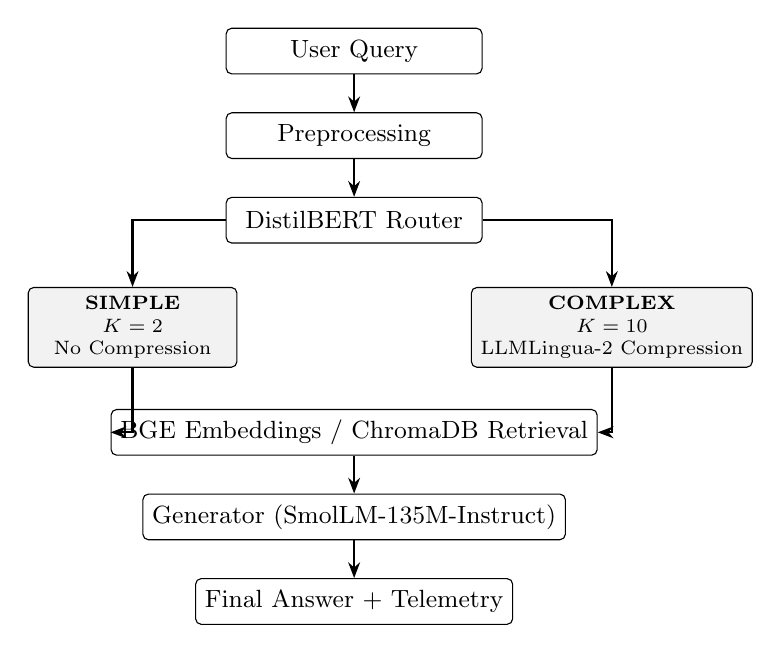
\begin{tikzpicture}[
node distance=0.48cm and 0.35cm,
block/.style={rectangle, draw, text centered, minimum width=3.25cm, minimum height=0.58cm, font=\small, rounded corners=2pt},
branch/.style={rectangle, draw, text centered, minimum width=2.65cm, minimum height=0.72cm, font=\scriptsize, align=center, rounded corners=2pt},
arrow/.style={-{Stealth[length=2mm]}, thick}
]
\node[block] (query) {User Query};
\node[block, below=of query] (preproc) {Preprocessing};
\node[block, below=of preproc] (router) {DistilBERT Router};

\node[branch, fill=gray!10, below left=0.55cm and -0.15cm of router] (simple)
{\textbf{SIMPLE}\\$K=2$\\No Compression};
\node[branch, fill=gray!10, below right=0.55cm and -0.15cm of router] (complex)
{\textbf{COMPLEX}\\$K=10$\\LLMLingua-2 Compression};

\node[block, below=2.1cm of router] (retrieve) {BGE Embeddings / ChromaDB Retrieval};
\node[block, below=of retrieve] (gen) {Generator (SmolLM-135M-Instruct)};
\node[block, below=of gen] (answer) {Final Answer + Telemetry};

\draw[arrow] (query) -- (preproc);
\draw[arrow] (preproc) -- (router);
\draw[arrow] (router) -| (simple);
\draw[arrow] (router) -| (complex);
\draw[arrow] (simple) |- (retrieve);
\draw[arrow] (complex) |- (retrieve);
\draw[arrow] (retrieve) -- (gen);
\draw[arrow] (gen) -- (answer);
\end{tikzpicture}
\caption{AdaptiveRAG system architecture. Query complexity directly determines retrieval depth and compression activation before the shared retrieval and generation stages.}
\label{fig:architecture}
\end{figure}

\subsection{Query Preprocessing}
The preprocessor validates that the query is non-empty and performs basic text normalization such as whitespace stripping. The original query is retained for experiment logging and evaluation. Preprocessing does not make routing decisions.

\subsection{Query Complexity Router}
The router is a fine-tuned binary classifier. It receives the normalized query text and outputs a complexity label and confidence score. We evaluated both \texttt{distilbert-base-uncased} and \texttt{bert-base-uncased} for this role, ultimately selecting DistilBERT due to its higher recall and lower routing latency in the controlled comparison.

The original DistilBERT router was trained for three epochs with batch size 16 and learning rate $2\times10^{-5}$. The alternative BERT router was trained for two epochs with batch size 8 and the same learning rate. Both experiments used seed 42, the same labeled data, preprocessing, evaluation data, and maximum sequence length.

Because complexity labels are inherited from dataset identity, router accuracy may partially reflect dataset-specific writing style rather than dataset-independent complexity understanding. This is discussed in Section~\ref{sec:limitations}.

\subsection{Retrieval}
\texttt{BAAI/bge-small-en-v1.5} produces 384-dimensional embeddings for queries and corpus chunks. ChromaDB performs cosine-similarity search over the persistent vector index. The same corpus, embedding model, and vector index are used across all retrieval-based strategies.

\subsection{Selective Context Compression}
Compression is enabled only for the COMPLEX route. The compressor is \texttt{microsoft/llmlingua-2-bert-base-multilingual-cased-meetingbank}, configured with a budget of 0.5 \cite{pan2024llmlingua2}.

A critical implementation correction was required during development. The initial design concatenated all retrieved chunks before compression, but $K=10$ commonly produced more than 512 tokens, exceeding the effective input limit of the compressor's underlying BERT model. The final implementation compresses each retrieved chunk independently and then concatenates the compressed outputs. This respects the per-call sequence-length constraint, although compression cost scales approximately linearly with $K$.

When compression fails, the original context is preserved and generation continues with the uncompressed evidence. The failure is recorded in execution metadata.

\subsection{Answer Generation}
All strategies use \texttt{HuggingFaceTB/SmolLM-135M-Instruct}. The common prompt is:
\begin{verbatim}
Question:
{query}

Context:
{context}
\end{verbatim}
The recorded generation configuration uses temperature 0.1, \texttt{max\_new\_tokens}=256, sampling enabled, and seed 42. The model was selected for CPU-only feasibility and reproducibility, not for state-of-the-art QA quality.

\section{Experimental Setup}

\subsection{Datasets and Splits}
The experiments use PopQA as a relatively simple factual proxy and HotpotQA as a complex multi-hop proxy \cite{mallen2023trust,yang2018hotpotqa}. The project uses 160 training samples, 40 development samples, a 298-sample router evaluation artifact used for classifier assessment, and a strictly held-out 10-query end-to-end benchmark consisting of five PopQA and five HotpotQA queries.

The 10-query benchmark was not used for router training or tuning.

\subsection{Corpus Construction}
The corpus uses a fixed 512-token chunk size with 50-token overlap. Chunks are embedded with \texttt{BAAI/bge-small-en-v1.5} and stored in a persistent ChromaDB collection using cosine similarity. The same indexed corpus is reused across retrieval-based baselines.

\subsection{Baselines}
Four strategies are compared:

\begin{table}[t]
\centering
\small
\caption{Baseline Strategies}
\label{tab:baselines}
\begin{tabular}{lcccc}
\toprule
Strategy & Retrieval & $K$ & Compression & Router\\
\midrule
LLM-only & No & 0 & No & No\\
Fixed RAG & Yes & 5 & No & No\\
Always-Compress & Yes & 10 & Yes & No\\
AdaptiveRAG & Yes & 2/10 & Conditional & Yes\\
\bottomrule
\end{tabular}
\end{table}

LLM-only measures generation without retrieval. Fixed RAG represents a conventional fixed retrieval policy. Always-Compress holds retrieval at $K=10$ and always compresses. AdaptiveRAG changes $K$ and compression according to the router output.

\subsection{Fairness Controls}
All four strategies use identical benchmark queries, corpus, chunking, embeddings, vector index, generator, prompt template, generation parameters, random seed, and evaluation code. The intended difference is the execution policy rather than model or infrastructure changes.

\subsection{Evaluation Metrics}
Answer quality is measured using Exact Match (EM) and token-level F1 after normalization of case, punctuation, articles, and whitespace. Efficiency is measured using retrieval, compression, generation, and total latency, together with context token counts and token reduction. Router quality is measured using accuracy, macro precision, macro recall, macro F1, confusion matrix, and inference latency.

\section{Experimental Results}

\subsection{Classifier Comparison and Selection}
To evaluate router choice, we compared fine-tuned \texttt{distilbert-base-uncased} and \texttt{bert-base-uncased} on the same 298-sample router evaluation artifact.

\begin{figure}[t]
\centering
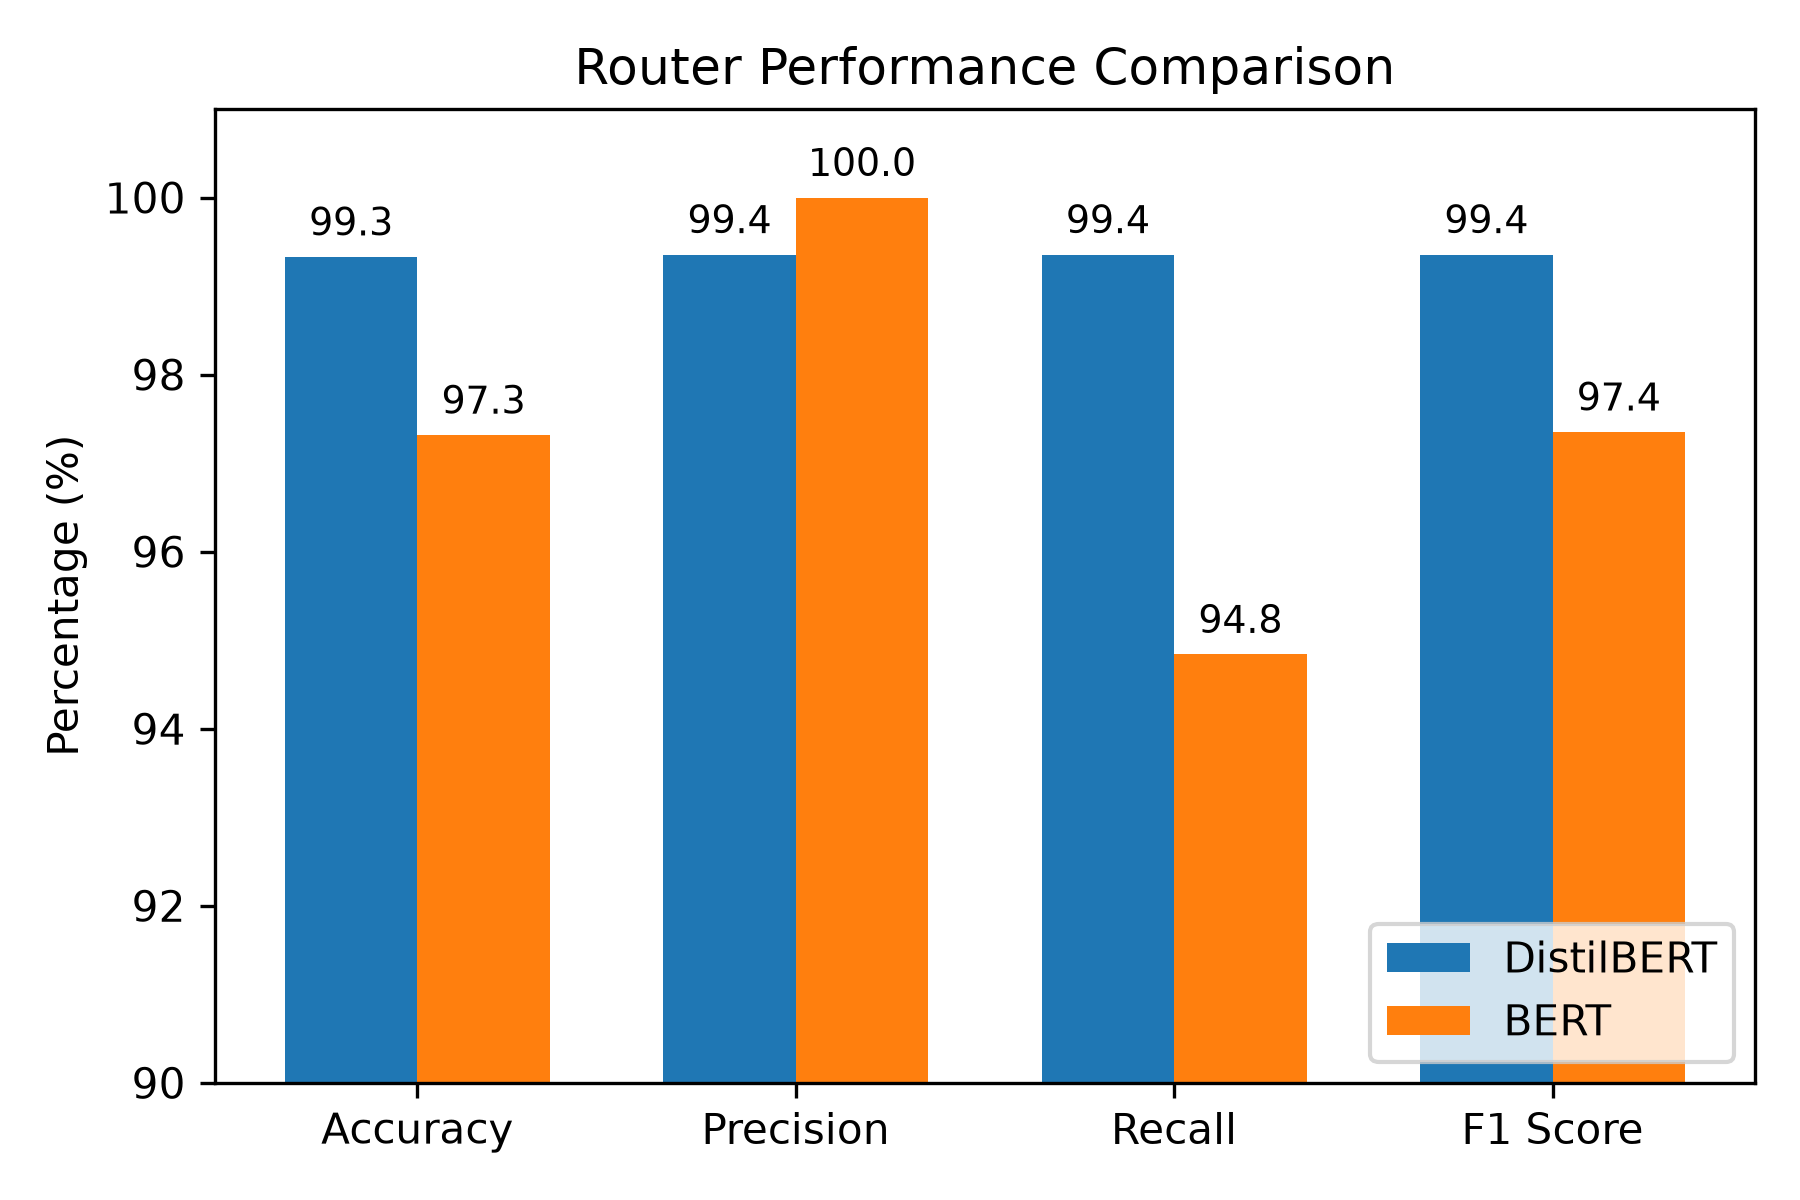
\includegraphics[width=0.86\linewidth]{figures/classifier_performance.png}
\caption{Classifier performance comparison between DistilBERT and BERT on the 298-sample evaluation set.}
\label{fig:classifier_perf}
\end{figure}

\begin{figure}[t]
\centering
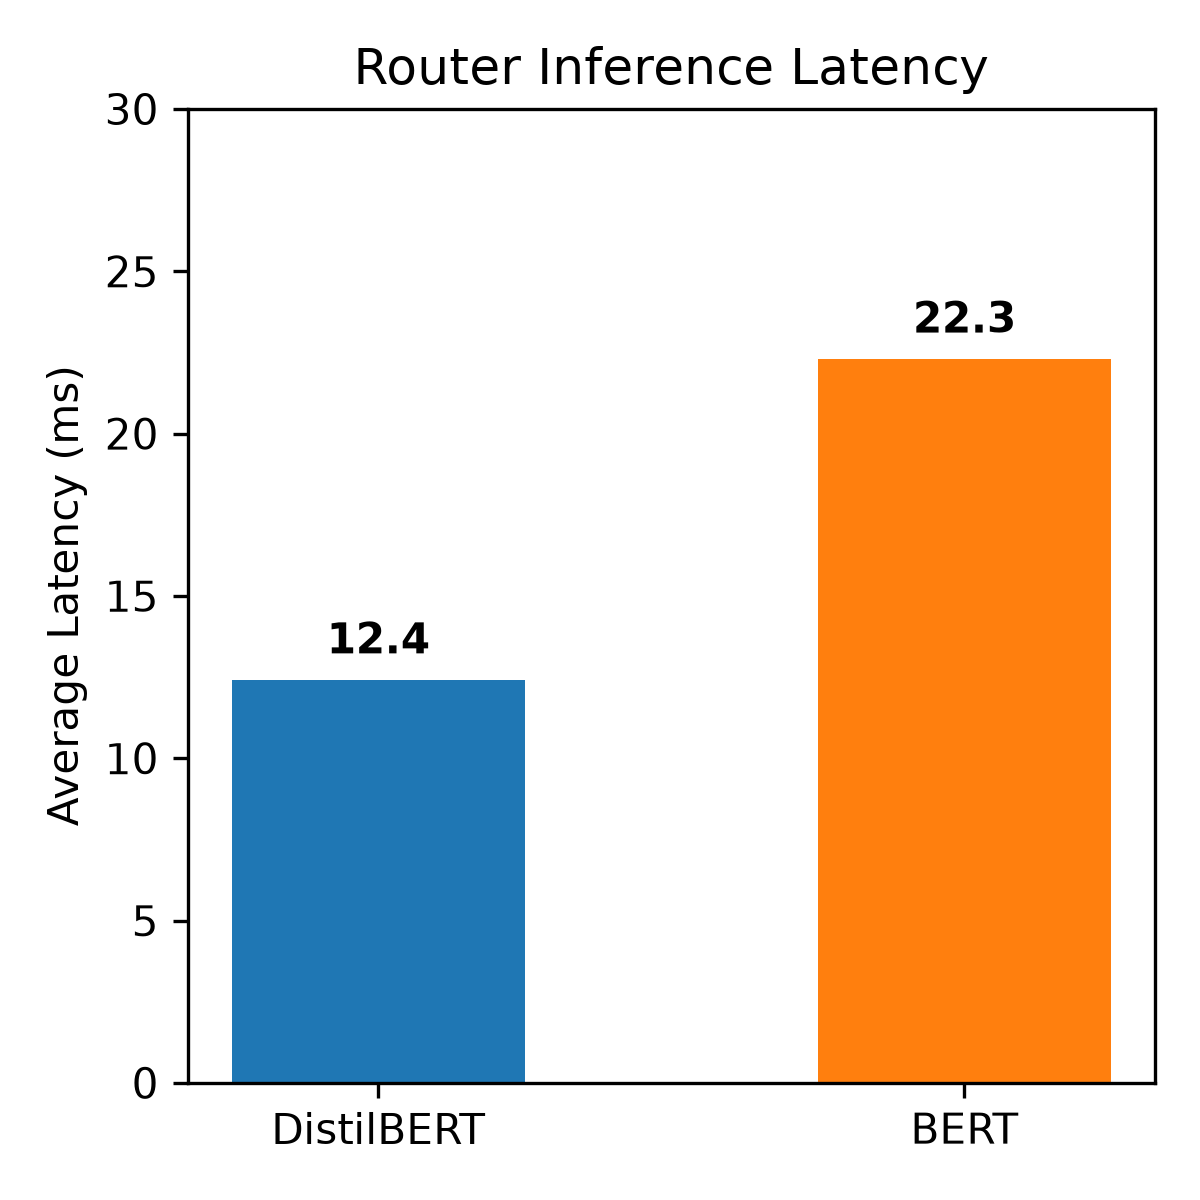
\includegraphics[width=0.70\linewidth]{figures/classifier_latency.png}
\caption{Inference latency comparison of the routing classifiers.}
\label{fig:classifier_lat}
\end{figure}

\begin{table}[t]
\centering
\small
\caption{Router Comparison on 298 Samples}
\label{tab:router_comp}
\begin{tabular}{lccc}
\toprule
Metric & DistilBERT & BERT & Difference\\
\midrule
Accuracy & 99.33\% & 97.32\% & $-2.01\%$\\
Precision & 99.35\% & 100.00\% & $+0.65\%$\\
Recall & 99.35\% & 94.84\% & $-4.51\%$\\
F1 & 99.35\% & 97.35\% & $-2.00\%$\\
Latency & 12.42\,ms & 22.30\,ms & $+9.88$\,ms\\
False Negatives & 1 & 8 & $+7$\\
\bottomrule
\end{tabular}
\end{table}

DistilBERT was better suited to this experimental setup based on higher accuracy, recall, F1, and lower routing latency. BERT failed to recall 8 COMPLEX queries by labeling them SIMPLE, whereas DistilBERT missed only 1. In the AdaptiveRAG policy, a COMPLEX-to-SIMPLE error reduces retrieval from $K=10$ to $K=2$ and disables compression, potentially reducing the evidence available to the generator. DistilBERT was therefore selected for the primary benchmark.

\subsection{Primary Benchmark}
The primary end-to-end benchmark uses the DistilBERT router on the ten-query held-out set.

\begin{figure}[t]
\centering
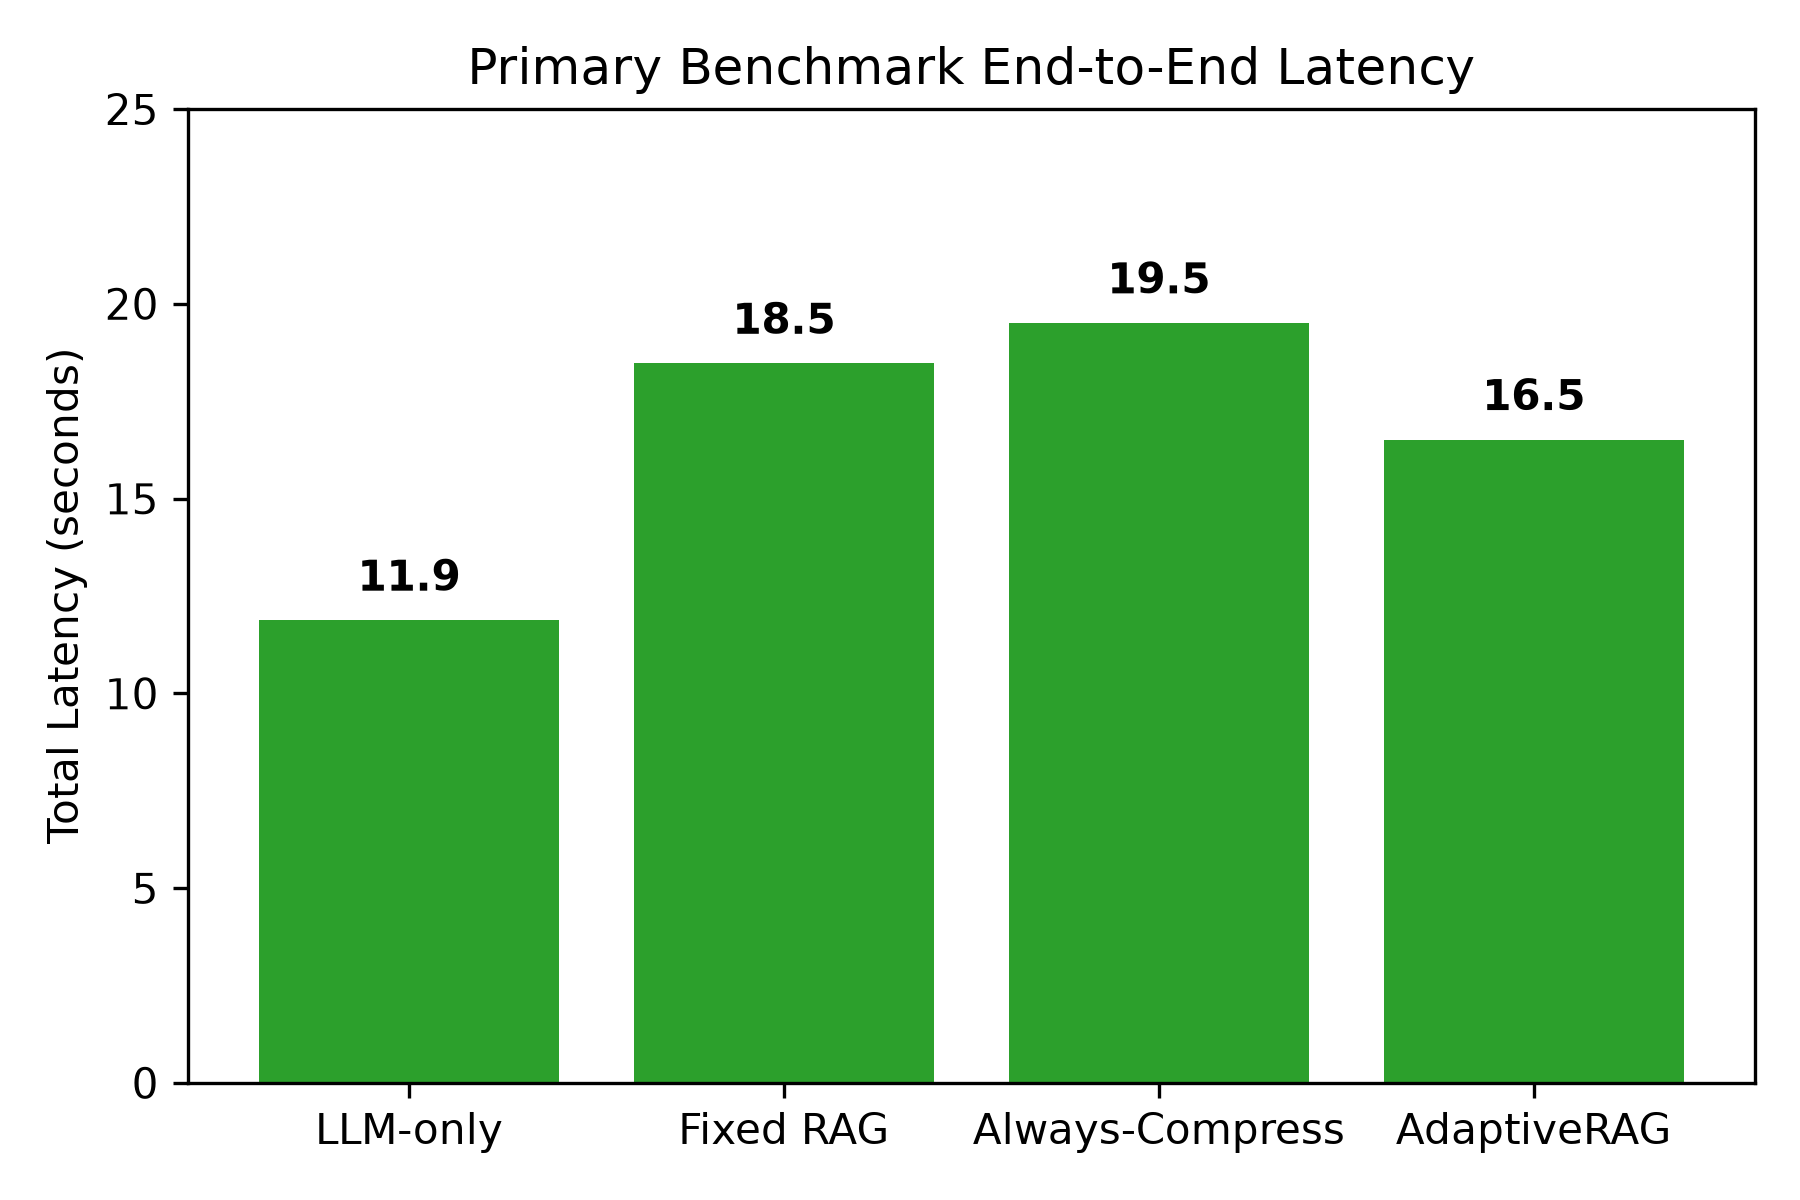
\includegraphics[width=0.94\linewidth]{figures/benchmark_latency.png}
\caption{Total end-to-end latency across the four benchmark strategies.}
\label{fig:benchmark_lat}
\end{figure}

\begin{table}[t]
\centering
\small
\caption{Primary Benchmark Results (10 Queries)}
\label{tab:benchmark}
\begin{tabular}{lccccc}
\toprule
Strategy & EM & F1 & Ret. & Gen. & Total\\
\midrule
LLM-only & 0.000 & 0.00146 & 0 & 11874 & 11877\\
Fixed RAG & 0.000 & 0.00577 & 805 & 17661 & 18472\\
Always-Compress & 0.000 & 0.00320 & 36 & 17890 & 19510\\
AdaptiveRAG & 0.000 & 0.00320 & 28 & 15679 & 16514\\
\bottomrule
\end{tabular}
\end{table}

All strategies obtain EM $=0.0$, and Token F1 is extremely low. Among retrieval-augmented strategies, AdaptiveRAG achieves the lowest observed total latency at 16.514\,s, compared with 18.472\,s for Fixed RAG and 19.510\,s for Always-Compress. These results demonstrate an efficiency pattern rather than an answer-quality advantage. The router overhead is small relative to generation latency.

\subsection{Downstream Classifier Effect}
To measure the end-to-end impact of the alternative classifier, the AdaptiveRAG pipeline was run with the BERT router on the identical ten-query held-out benchmark. Both models made the same ten routing decisions: all five PopQA queries were classified as SIMPLE and all five HotpotQA queries as COMPLEX. Consequently, they selected the same retrieval depths and compression behavior on this small benchmark. The observed downstream quality difference is small and cannot establish a meaningful answer-quality difference on ten queries. This also shows why the larger 298-sample router evaluation is necessary for exposing routing edge cases.

\section{Compression Ablation Study}

To isolate the contribution of compression, a controlled ablation compares two conditions using identical $K=10$ retrieval, the same ten queries, and the same configuration.

\begin{figure}[t]
\centering
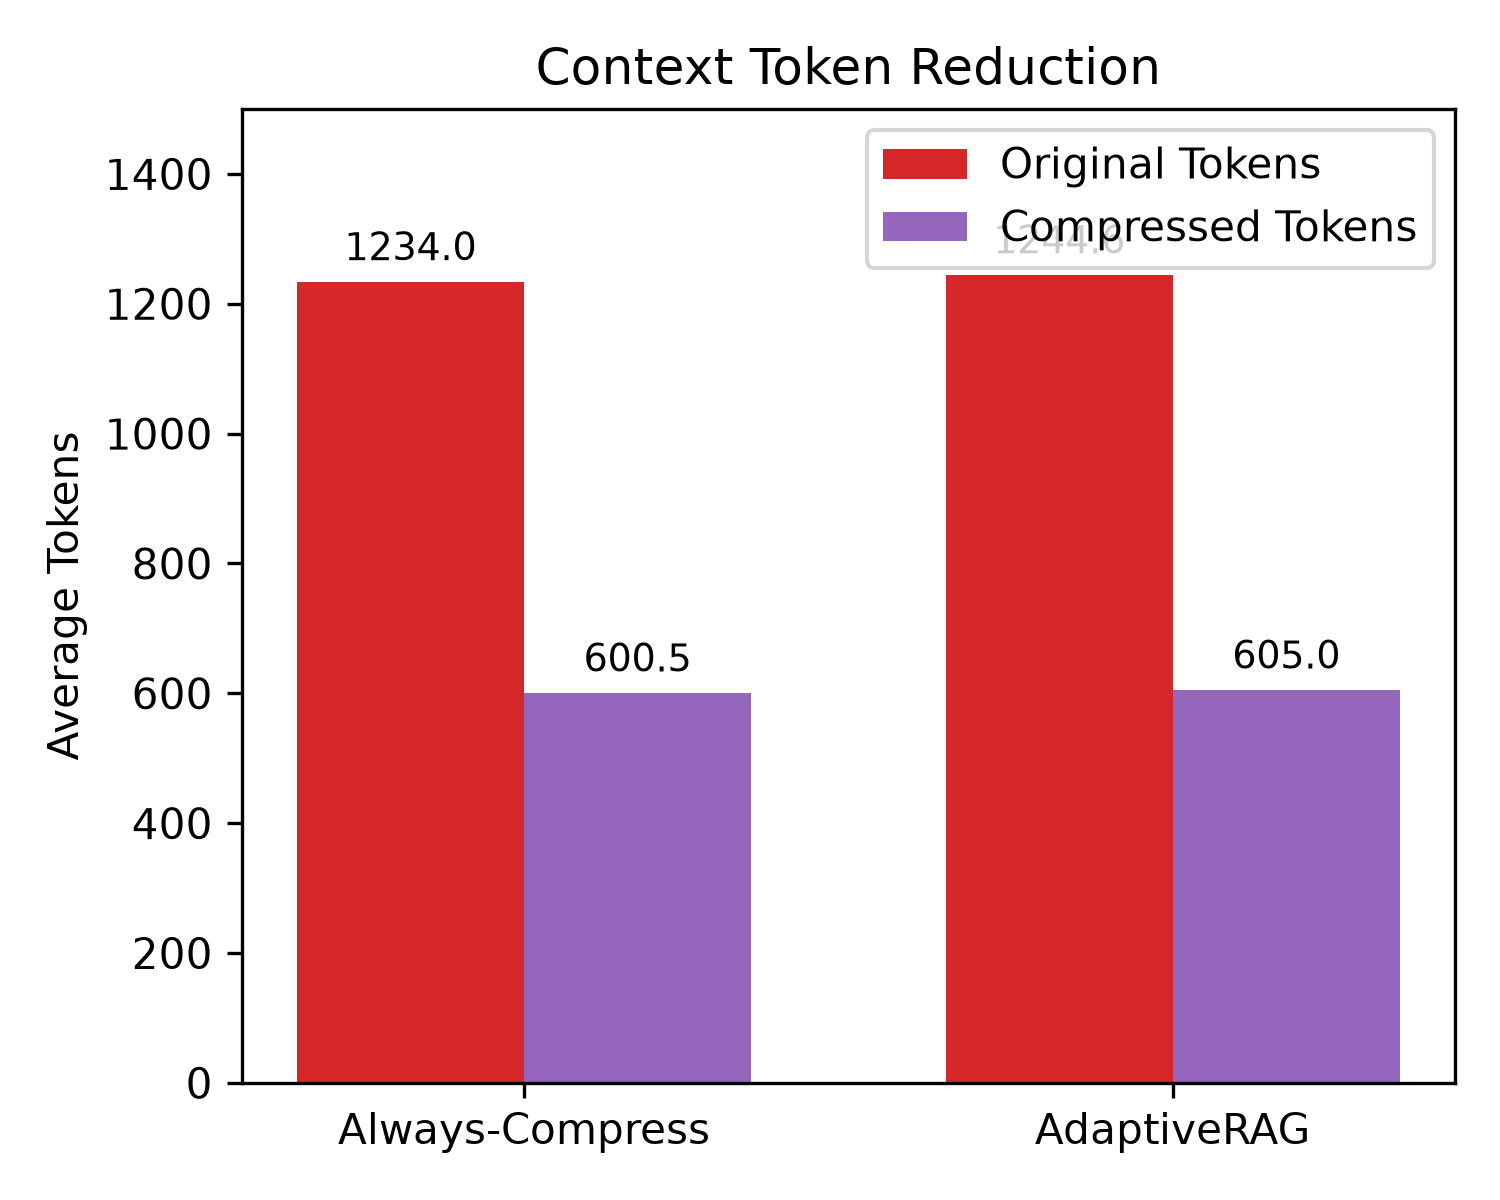
\includegraphics[width=0.82\linewidth]{figures/token_reduction.png}
\caption{Context token reduction produced by LLMLingua-2 compression.}
\label{fig:token_red}
\end{figure}

\begin{table}[!t]
\centering
\small
\caption{Compression Ablation ($K=10$, 10 Queries)}
\label{tab:ablation}
\begin{tabular}{lcc}
\toprule
Metric & No Compr. & With Compr.\\
\midrule
EM & 0.000 & 0.000\\
Token F1 & 0.00473 & 0.00351\\
Orig. Tokens & --- & 1233.9\\
Compr. Tokens & --- & 598.9\\
Token Reduction & --- & 51.46\%\\
Avg. Compr. Lat. (ms)$^*$ & 0 & 13488\\
Avg. Gen. Lat. (ms) & 77079 & 55660\\
Avg. Total Lat. (ms)$^{**}$ & 78838 & 70032\\
\bottomrule
\multicolumn{3}{l}{\scriptsize $^*$ Compression latency averaged over compression-enabled queries only.}\\
\multicolumn{3}{l}{\scriptsize $^{**}$ Total latency averaged over the complete benchmark run.}
\end{tabular}
\end{table}

Compression removes approximately 635 tokens per query on average, corresponding to a 51.46\% reduction in observed context length. Generation latency decreases by 21.419\,s, while compression adds 13.488\,s. The measured total latency consequently decreases by 8.806\,s. This favorable balance is specific to the CPU execution environment and the slow generator.

Answer quality does not improve in this ablation: EM remains zero and Token F1 decreases from 0.00473 to 0.00351. With only ten examples and a weak generator, this change is descriptive rather than statistically meaningful.

\section{Error Analysis and Limitations}
\label{sec:limitations}

\subsection{Generator Bottleneck}
The strongest limitation is the generator. SmolLM-135M-Instruct was selected because the project required local CPU execution, but it frequently failed to produce concise correct answers. Across all primary strategies, EM is zero and Token F1 is extremely low. Consequently, the current experiments cannot establish whether one retrieval/compression policy improves factual answer quality over another.

\subsection{Proxy Complexity Labels}
The router labels are derived from dataset membership: PopQA is treated as SIMPLE and HotpotQA as COMPLEX. This makes the classification task easier than genuine complexity estimation and creates a risk that the router learns dataset-specific stylistic features. The 99.33\% router score should therefore be interpreted as performance on the proxy classification task rather than universal complexity understanding.

\subsection{Small End-to-End Benchmark}
The primary benchmark contains only ten queries, which is sufficient for a functional controlled demonstration but insufficient for reliable statistical significance testing or broad generalization. The identical downstream routing behavior of the two classifiers illustrates this limitation.

\subsection{Compression Sequence-Length Constraint}
The LLMLingua-2 compressor used in this implementation has a 512-token sequence-length constraint. The original concatenated compression approach was therefore invalid for many $K=10$ inputs. Chunk-wise compression fixes the input-length issue but may reduce globally coordinated compression and causes compression cost to scale with $K$.

\subsection{CPU-Only Execution}
The reported absolute latency values are strongly affected by CPU inference. In particular, slow generation makes context reduction disproportionately valuable in the ablation. Faster hardware may produce a different balance between compression cost and generation savings.

\subsection{Generalizability}
The measured behavior depends on the selected datasets, corpus construction, embeddings, generator, compressor, retrieval values, and hardware. The results therefore describe a controlled local prototype rather than a universal property of adaptive RAG systems.

\section{Discussion}

The experiments establish three main observations. First, a lightweight classifier can add a routing decision at very small computational cost relative to the generator: the controlled classifier comparison records 12.42\,ms average inference latency for DistilBERT. Second, the deterministic controller creates distinct shallow and deep execution paths, and the shallow path is associated with lower generation latency in the ten-query AdaptiveRAG sample. Third, context compression can substantially reduce the amount of text presented to the generator, but the overall value of compression depends on the downstream generator's cost.

The primary benchmark should be interpreted carefully. AdaptiveRAG has lower observed latency than the fixed retrieval-based baselines, but the experiment does not establish a quality improvement: all strategies obtain EM $=0.0$ and very low Token F1. In this environment, the main measurable effect of adaptation is therefore computational routing rather than answer-quality enhancement.

The compression ablation is also configuration-dependent. The observed 8.806\,s total-latency reduction results from a specific combination of 51.46\% context reduction, 13.488\,s compression overhead, and 21.419\,s generation-time savings. With a faster generator, the same compression process may no longer be economically attractive.

\section{Conclusion and Future Work}

This paper presented AdaptiveRAG, a query-complexity-aware RAG prototype that uses a lightweight classifier to select between a shallow $K=2$ retrieval path without compression and a deep $K=10$ path with LLMLingua-2 compression. The system was compared with LLM-only, Fixed RAG, and Always-Compress baselines under shared infrastructure.

The router comparison shows that DistilBERT was better suited to this experimental setup than the tested BERT alternative, achieving 99.33\% accuracy and 99.35\% F1 with 12.42\,ms average routing latency. On the ten-query held-out benchmark, AdaptiveRAG records 16.514\,s average total latency versus 18.472\,s for Fixed RAG and 19.510\,s for Always-Compress. The compression ablation produces 51.46\% token reduction and an observed 8.806\,s reduction in total latency.

However, all primary strategies yield EM $=0.0$, so the current experiments do not establish an answer-quality advantage for any policy. The small benchmark, proxy complexity labels, CPU-only execution, and weak generator are important limitations.

Future work includes replacing the generator with a substantially larger local model, evaluating hundreds or thousands of held-out queries, constructing complexity labels independently of dataset identity, testing on unseen datasets, sweeping $K$ more systematically, and evaluating the pipeline on GPU hardware. Confidence-aware routing is another promising direction.

\section*{Acknowledgment}
The authors thank Dr.\ Vijayaprabakaran K, Vellore Institute of Technology, Chennai, for faculty guidance and feedback during the development of this work.

\bibliographystyle{IEEEtran}
\bibliography{references}

\end{document}